\documentclass[main.tex]{subfiles}
\begin{document}

\section{Parsing and Classification}

\subsection{Choice of Language}

With very few exceptions, the code I wrote in support of this thesis was done in Clojure, a dialect of LISP designed to work on top of the Java Virtual Machine (JVM). The choice of a language was simple: a heavy dependence on the Stanford Parser and the WEKA package, both written in Java, necessitated a JVM-based language. The slowness of Java's compile/debug cycle eliminated that language as an option, leaving a handful of possible languages, from which I chose Clojure for its speed, functional style, and elegance.

\subsection{Parsing}

The Stanford Parser software package, version 1.6.7, configured with the included probabilistic context-free grammar (PCFG) \citep*{klein-manning-pcfg:2003}, was used to generate all syntactic parse trees and grammar dependency graphs. A detailed description of PCFGs is beyond the scope of this paper, and the reader who desires such is referred to \citet{booth:1973}. Central to the PCFG is the context-free grammar (or \textit{phrase structure grammar}). A context-free grammar consists of a number of rules each of which describe the various possible compositions of a particular type of phrase. For instance, Figure~\ref{fig:ps-rules} shows a very simple grammar consisting of five rules.
\begin{figure}
\centering
\begin{tabular}{l l l l}
a. & S & $\rightarrow$ & $\text{NP} \text{ VP}$\\ 
b. & NP & $\rightarrow$ & $(\text{Det}) \text{ N } (\text{PP})$\\
c. & VP & $\rightarrow$ & $(\text{Aux}) \text{ V } (\text{NP}) \text{ } (\text{AdvP})^n$\\
d. & PP & $\rightarrow$ & $\text{P } \text{NP}$\\
e. & AdvP &  $\rightarrow$ & $\begin{Bmatrix}
\text{Adv} \\ \text{PP} \\
\end{Bmatrix} $
\end{tabular}
\caption{Simple Phrase Structure Rules. \citep[Ch. 5.3]{akmajian:2010}}
\label{fig:ps-rules}
\end{figure}
Rule (a) indicates that a sentence (S) is composed of a noun phrase (NP) followed by a verb phrase (VP). Rule (b) says that a noun phrase is composed of a noun (N) preceded by an option determiner (Det) and followed by an option prepositional phrase (PP). Rule (c) says that a verb phrase contains an option auxiliary verb (Aux), followed by a verb (V), followed by an optional noun phrase and then by zero or more adverbial phrases (AdvP). A prepositional phrase is defined by rule (d) as being a preposition plus a noun phrase, and an adverbial phrase is defined by rule (e) as being either an adverb or a prepositional phrase. Again, these are only example rules and cover just a small subset of English grammar. Also, the symbols used by the Stanford parser are not necessarily the same used in these example rules. Using these rules, the sentence \textit{the sun will dry the grapes} can be represented as the tree shown in Figure~\ref{fig:ps-tree}.
\begin{figure}[htbp]
\centering
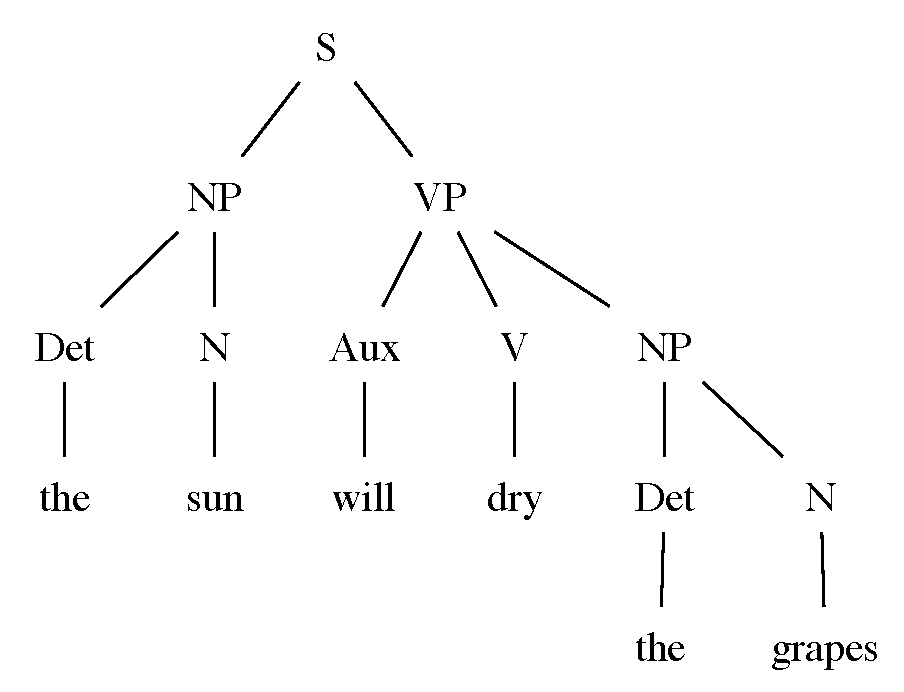
\includegraphics[scale=0.6]{ps-tree.pdf}
\caption{Parse of \textit{the sun will dry the grapes} Generated from Rules in Figure~\ref{fig:ps-rules}.}
\label{fig:ps-tree}
\end{figure}
Generating this graph from the original sentence requires a certain knowledge of the parts of speech of the words in the sentence. To some extent, it is not necessary to have all of this information. In fact, if any of the open-class words (i.e. the verb or the two nouns) in this example are replaced with nonsense words, most people would have no trouble parsing it and would generate a tree with same structure as that in Figure~\ref{fig:ps-tree}. Similarly, the Stanford parser successfully parses this sentence even if all of the open-class words are replaced with nonsense words. This does not always hold true for more complex sentences, and replacing the closed-class words with gibberish makes the sentence much more difficult to parse. Also, replacing one word with another word of a different part of speech (e.g. \textit{the sun will dry the warmly}) produces a sentence that is difficult to parse for both human and computer. Parsers guess the part of speech of unknown words the same way humans do, by choosing whatever part of speech produces the most common valid phrase structure. Parsers use a similar method for dealing with ambiguities.

Consider the sentence \textit{the bag was found in the woods by a farmer}. Using the phrase rule structures from Figure~\ref{fig:ps-rules}, one could generate either the parse shown in Figure~\ref{fig:ps-tree-ambig1} or that shown in Figure~\ref{fig:ps-tree-ambig2}. 
\begin{figure}[htbp]
\centering
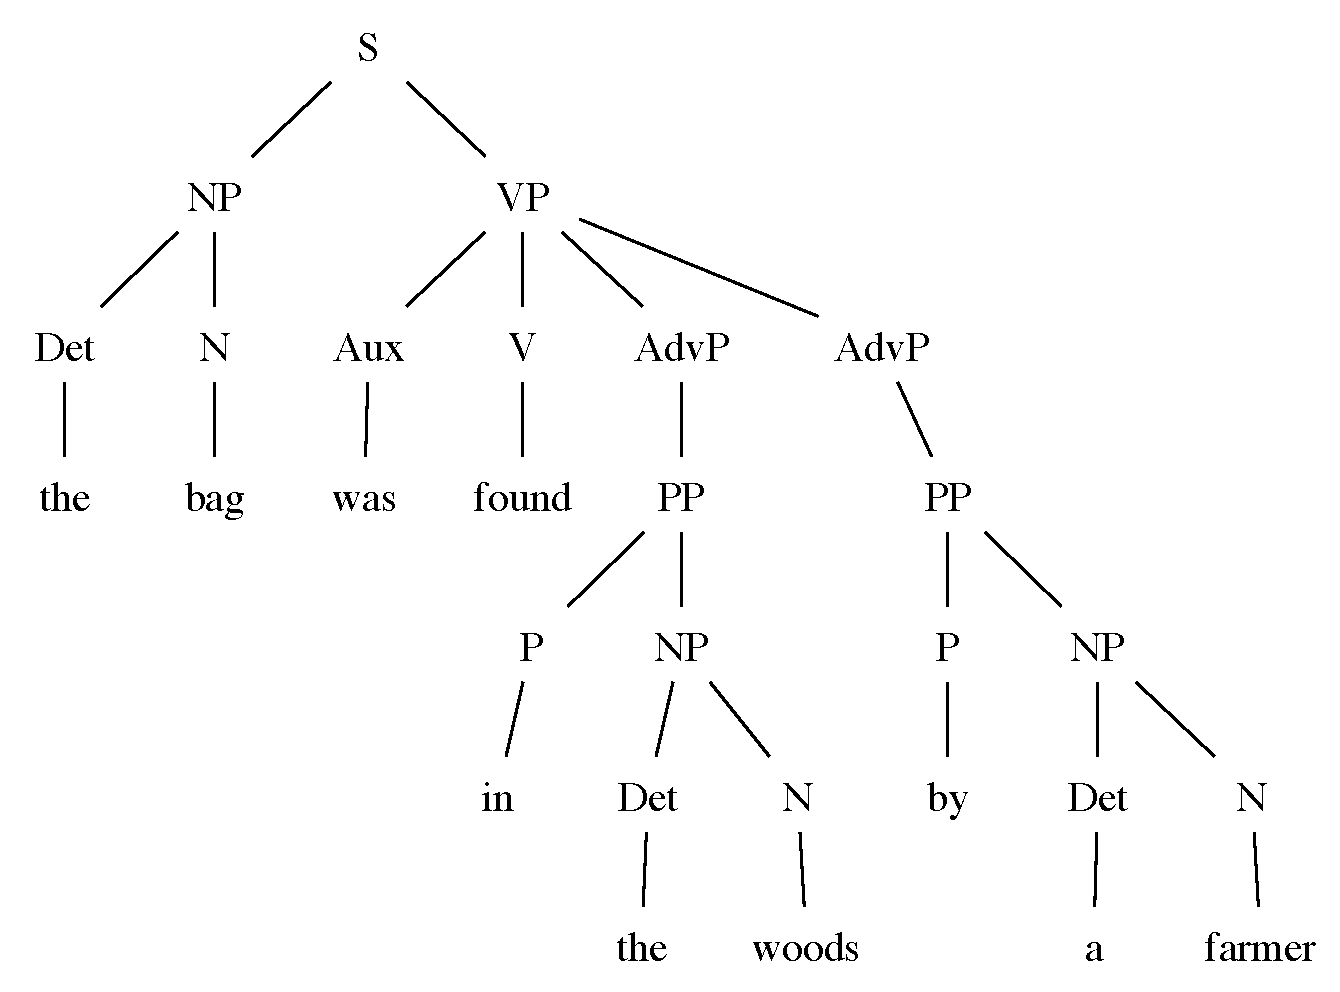
\includegraphics[scale=0.6]{ps-tree-ambig1.pdf}
\caption{Possible Parse of \textit{the bag was found in the woods by a farmer} Generated from Rules in Figure~\ref{fig:ps-rules}.}
\label{fig:ps-tree-ambig1}
\end{figure}
\begin{figure}[htbp]
\centering
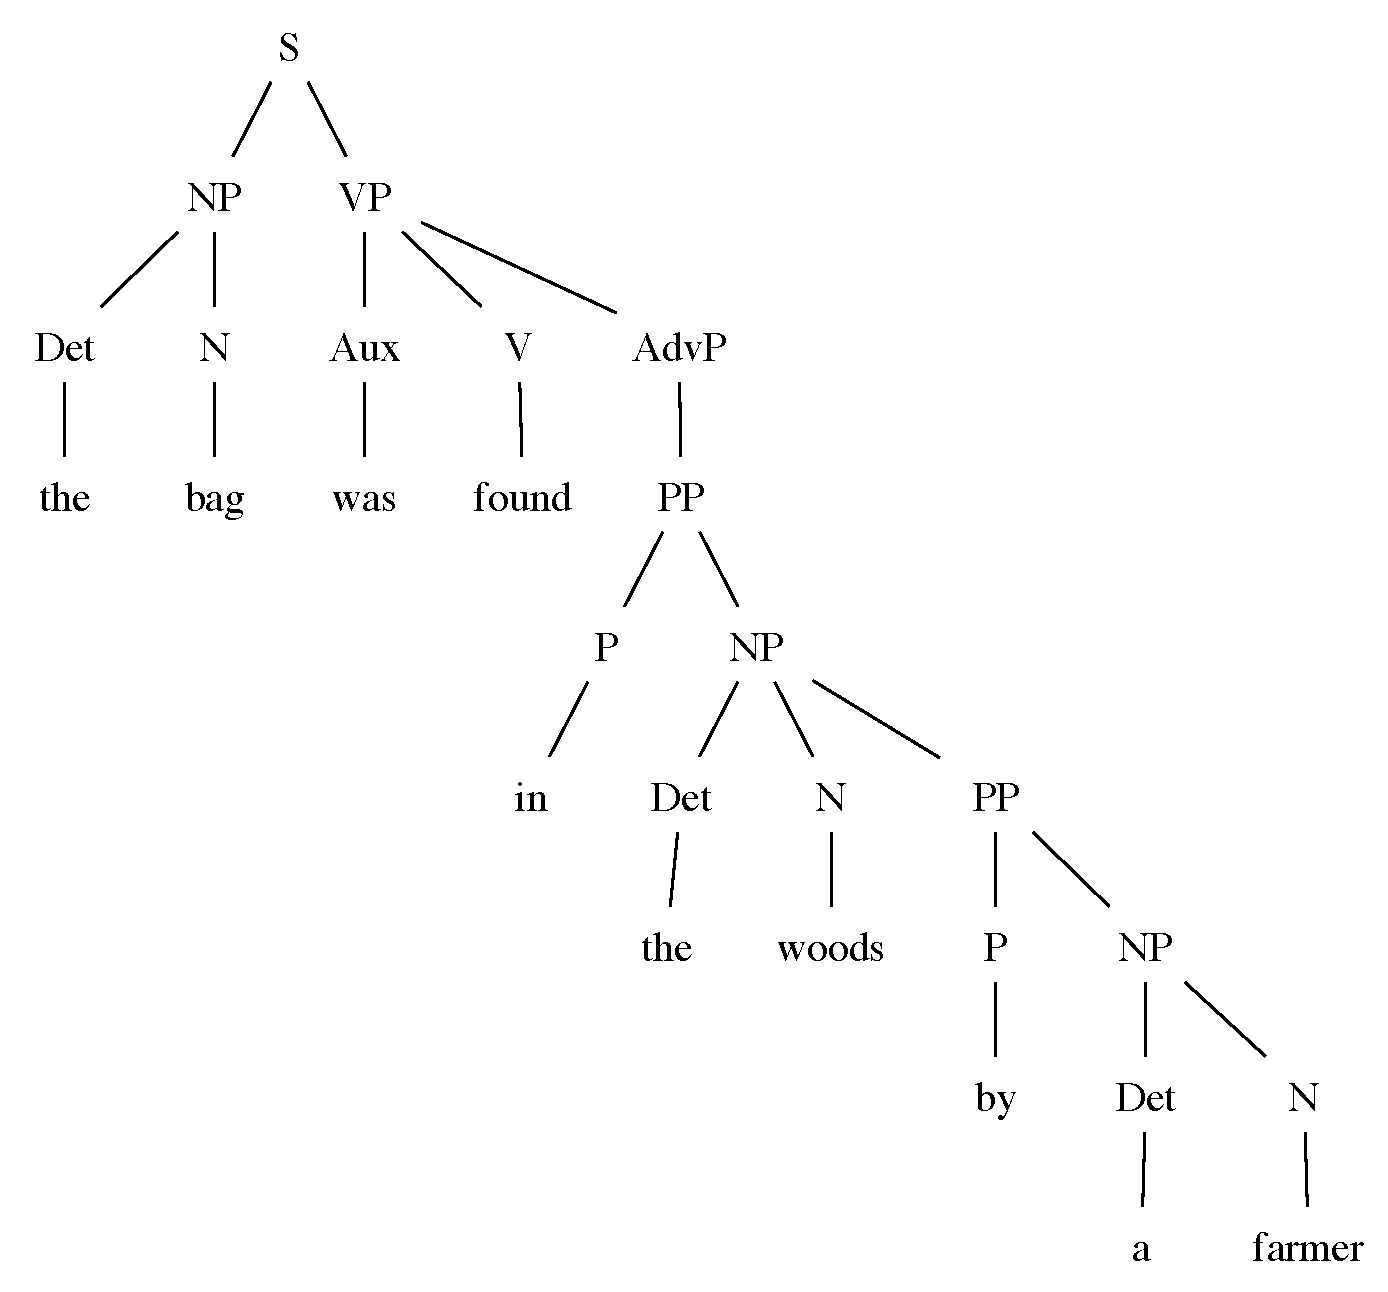
\includegraphics[scale=0.6]{ps-tree-ambig2.pdf}
\caption{Possible Parse of \textit{the bag was found in the woods by a farmer} Generated from Rules in Figure~\ref{fig:ps-rules}.}
\label{fig:ps-tree-ambig2}
\end{figure}
In both parses, the PP \textit{in the woods} is considered an adverbial phrase modifying the verb. However, the second PP can be parsed either the same way, or it can be placed within the NP containing \textit{woods}. In other words, the sentence can either mean that a farmer found the bag, or that the bag was found in the woods and those woods were located near a farmer. The first interpretation is the one that most English speakers would choose based on the semantic content of the two options. A rule-based parser, however, is unable to attempt semantic interpretation, and a purely rule-based parser might output all possible interpretations. A PCFG-based parser, however, will choose the parse that is \textit{statistically} most likely to be correct. Such a parser requires a large database of correct parses with which it can make probability measurements. The Stanford parser, for instance, uses the Penn Treebank, a corpus of parsed English texts \citep{marcus:1993}. Out of the various possible parses, the one that a probabilistic parser will choose is the one that has a structure, or a substructure, that is common among parses in the database. The parser does not include only the phrase structure in its consideration, but to a certain extent it includes the words itself. For instance, given \textit{the bag was found in the woods by a farmer}, the Stanford Parser will generate a parse very similar to Figure~\ref{fig:ps-tree-ambig1}. However, when given the sentence \textit{the bag was found under the bridge over the stream}, which has the same two possible parses, it chooses the other, the semantically correct one. At first impression, one might think that the parser had located a semantic connection between \textit{bridge} and \textit{stream}, and had used this to choose the correct parse. However, it turns out that it is actually the prepositions (a group of closed-class words) that cause the difference in parsing. For instance, the sentence \textit{the bag was found under the woods over a farmer}, is parsed like Figure~\ref{fig:ps-tree-ambig2} and \textit{the bag was found in the bridge by the stream} is parsed like Figure~\ref{fig:ps-tree-ambig1}. Hence the parser does not consider the open-class (content) words nearly so much as it does the closed-class (structure) words, when choosing between parses.

\subsection{The Tests}
The crux of this project was the design and creation of a suite of tests, each of which identifies a number of closely related grammatical characteristics of the text samples. These tests operate on the output from the Stanford parser, i.e. parse trees and grammatical dependencies. As output they generate training or testing cases to be used by the Weka classifier. Each of these cases consists of multiple attributes, corresponding to grammatical features, each with continuous values indicating the relative frequency (probability) of that particular feature. For a case with $n$ attributes where the number of occurrences of the grammatical feature associated with the $i$th attribute is $g_i$, the value $f_i$ for that attribute is given by $g_n  / \displaystyle\sum\limits_{i=1}^n g_i$. For instance, one test measures the relative frequencies of the various tense/aspect/voice combinations of finite verbs. English has twenty-four such combination, so the case generated by this test has twenty-four attributes.

In addition to the attributes, each case has a class which can be \textit{es} or \textit{en}, indicating that the class is associated with a text sample written by an L1-Spanish speaker or by a native English speaker, respectively. For training cases, the classes are known beforehand and are assigned to the cases manually. For testing cases, the classes have missing values, until such values are determined by a classifier, as discussed in the following section.

\subsection{Classification}

I used the Weka machine learning package, version 3.6 \citep{hall-et-al:2009}, to create, train and test classifiers based on the cases discussed above. I primarily used two classifiers: J48, which is Weka's implementation of the C4.5 classifier \citep*{quinlan:1993} and the RandomForest classifier, which is based on the random forest algorithm described by \citet{breiman:2001}. The former is useful for its highly readable decision trees, which clearly indicate which attributes are involved in the classification and their roles. In later sections of this paper are found linguistic explanations for why these particular attributes should be useful in classification.
 
\subsubsection{C4.5}

This section describes the C4.5 partition as it applies to this project. That is to say, C4.5 can deal with a number of circumstances that do not arise here. What is described here is a version of the C4.5 algorithm that is restricted to continuous attribute values and to exactly two class values, and which does not permit missing attribute values. That having been said, the C4.5 algorithm consists of two phases, \textit{tree construction} and \textit{tree pruning}.

In the tree construction phase a decision tree is built which successively performs binary partitioning of a set of training cases. Consider a full binary tree where each edge represents a set of cases and each non-terminal node a partitioning operation, as shown in Figure~\ref{fig:c45-dtree}. These partitioning operations take one set, represented by the parent edge, and divide it into two subsets, the daughter edges. The root node operates on an initial set $S_0$, and a leaf node simply indicates that its parent edge is a set consisting of cases of a single class. Let the first partitions of $S_0$ be called $S_1$ and $S_2$ where $S_1\cup S_2 = S_0$ and $S_1\cap S_2 = \emptyset$ , and of $S_1$ let them be called $S_{1,1}$ and $S_{2,1}$ and so forth. Likewise, let the partitioning operation that operates on a particular set be designated by $T$ with the same subscripts as that set.
\begin{figure}
\caption{A decision tree showing the partitioning of a set of training cases $S_0$ into subsets $S_{1,2}$, $S_{1,1,1}$, and $S_{1,2,1}$ whose elements are of class $C_1$, and $S_{2,2}$, $S_{2,1,1}$, and $S_{2,2,1}$ whose elements are of class $C_2$. The nodes $T_0$, $T_1$, etc. are partitioning operations such that for any operation $T$ operating on a set $S_a$ the generated sets are $S_{1,a}$ and $S_{2,a}$ where $S_{1,a}\cup S_{2,a} = S_a$ and $S_{1,a}\cap S_{2,a} = \emptyset$.}
\[ \xygraph{ !{<0cm,0cm>;<1cm,0cm>:<0cm,1cm>::}
!{(4,9)}*+{}="O"
!{(4,8) }*+{T_0}="t"
!{(1,7) }*+{T_1}="t1"
!{(6,7) }*+{T_2}="t2"
!{(-1,6)}*+{T_{1,1}}="t11"
!{(3,6)}*+{T_{2,1}}="t21"
!{(-2,5)}*+{C_1}="l1"
!{(-0,5)}*+{C_2}="l2"
!{(2,5)}*+{C_1}="l3"
!{(4,5)}*+{C_2}="l4"
!{(5,6)}*+{C_1}="l5"
!{(7,6)}*+{C_2}="l6"
"O":"t" _{\tiny $S_0$}
"t":"t1" _{\tiny $S_1$}
"t":"t2" ^{\tiny $S_2$}
"t1":"t11" _{\tiny $S_{1,1}$}
"t1":"t21" ^{\tiny $S_{2,1}$}
"t2":"l5" _{\tiny $S_{1,2}$}
"t2":"l6" ^{\tiny $S_{2,2}$}
"t11":"l1" _{\tiny $S_{1,1,1}$}
"t11":"l2" ^{\tiny $S_{2,1,1}$}
"t21":"l3" _{\tiny $S_{1,2,1}$}
"t21":"l4" ^{\tiny $S_{2,2,1}$}
 } \]

\label{fig:c45-dtree}
\end{figure}

The partitioning operations are performed by applying a binary test to each case within $S$, the set to be partitioned, and dividing the set based on the results. Each test considers a single attribute $A$ and compares the value of that attribute, $V_A$, to a threshold value, $V_C$. All cases where the $V_A\leq V_C$ will be put into one subset and all other cases into the other.

The decision of the attribute and threshold value for a particular test is determined using what Quinlan calls the ``gain ratio criterion'' which is calculated as follows. If the probability of randomly drawing a case of class $C_1$ from a set $S$ is $p_1$ and of drawing a case of the other class is $p_2$ where $p_2 = 1-p_1$, then the average amount of information needed to identify the class of a case in $S$ can be defined in terms of entropy as
\[
\mathrm{info}(S)=-p_1 \cdot \log_2(p_1) - p_2 \cdot \log_2(p_2).
\]
A similar measure can be applied to the two partitions $S_1$ and $S_2$ created by applying the partitioning test $T$ to $S$. The entropy after partition is given by taking a weighted sum of the entropy of the two sets as
\[
\mathrm{info}_T(S)=\frac{|S_1|}{|S|} \cdot \mathrm{info}(S_1) + \frac{|S_2|}{|S|} \cdot \mathrm{info}(S_2)
\]
The decrease in entropy, expressed as a positive value (an information gain), due to partitioning $S$ using the test $T$ is then
\[
\mathrm{gain}(T)=\mathrm{info}(S)-\mathrm{info}_T(S).
\]
Maximizing this gain can be and, in ID3 the predecessor to C4.5, was used as measurement of test fitness. However, in the more general case of C4.5, where one test can partition a set into more than 2 subsets, using this gain criterion to choose tests favors tests that partition sets into numerous subsets. To mitigate this, Quinlan added another factor to the criterion, the split info which for this special case is given by
\[
\mathrm{split\ info}(T)= -\frac{|S_1|}{|S|} \cdot \log_2 \left( \frac{|S_1|}{|S|} \right) - \frac{|S_2|}{|S|} \cdot \log_2  \left( \frac{|S_2|}{|S|}  \right).
\]
Then the fitness of a test $T$ can be measured using
\[
\mathrm{gain\ ratio}(T) = \frac{\mathrm{gain}(T)}{\mathrm{split\ info}(T)}
\]
It should be noted that in this special case where partitioning operations are always binary, the gain ratio criterion favors tests that split $S$ into disparately sized sets, as split info is at its maximum (unity) when $|S_1|=|S_2|$.

In choosing a test $T$, the C4.5 algorithm tries each attribute $A$ from the set $S$ of cases to be partitioned. For each, it orders the cases in $S$ on the value of $A$. If the values of $A$ corresponding to this ordered set are $\{v_1,v_2,\ldots,v_m\}$, then any threshold between $v_i$ and $v_{i+1}$ will result in the same partitions. From this it can be seen that the total number of possible partitions is $m-1$. The algorithm tries all such partitioning schemes, measuring the gain ratio of each. When an optimal attribute and corresponding partitioning scheme has been chosen, the algorithm than chooses a threshold value that will produce this result. Again, to partition $S$ into two sets where the values for $A$ are $\{v_1,v_2,\ldots,v_i\}$ and $\{v_{i+1},v_{i+2},\ldots,v_m\}$, a threshold value $v_C$ must be chosen such that $v_i \leq v_C < v_{i+1}$. For this, it chooses the largest value for $A$ from the entire training set $S_O$ that does not exceed the midpoint of this range. 



\biblio
\end{document}